\subsection{Macroscopic Media (\textbf{L3, L4})}

\subsubsection{\hyperref[A Conducting Sphere at a Dielectric Boundary]{A Conducting Sphere at a Dielectric Boundary}}

A conducting sphere with radius $R$ and charge $Q$ sits at the origin of coordinates. The space outside the sphere above the $z=0$ plane has dielectric constant $\kappa_{1}$. The space outside the sphere below the $z=0$ plane has dielectric constant $\kappa_{2}$.

\begin{figure}[h]
	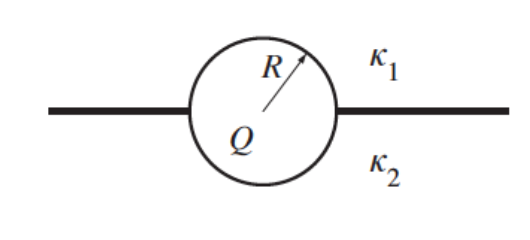
\includegraphics[width=6cm]{figures/spheredielectric.png}
	\centering
	\caption{Dielectric distribution around the sphere.}
\end{figure}

\begin{enumerate}
	\item  Find the potential everywhere outside the conductor.
	\item  Find the distributions of free charge and polarization charge wherever they may be.
\end{enumerate}

\subsubsection{\hyperref[Polarization by Superposition]{Polarization by Superposition}}

Two spheres with radius $R$ have uniform but equal and opposite charge densities $\pm \rho .$ The centers of the two spheres fail to coincide by an infinitesimal displacement vector $\delta$. Show by direct superposition that the electric field produced by the spheres is identical to the electric field produced by a sphere with a suitably chosen uniform polarization $\mathbf{P}$.

\subsubsection{\hyperref[The Field at the Center of a Polarized Cube]{The Field at the Center of a Polarized Cube}}

A cube is polarized uniformly parallel to one of its edges. Show that the electric field at the center of the cube is $\mathbf{E}(0)=-\mathbf{P} / 3 \epsilon_{0} .$ Compare with $\mathbf{E}(0)$ for a uniformly polarized sphere. Hint: Recall the definition of solid angle.

\subsubsection{\hyperref[E and D for an Annular Dielectric]{$\mathbf{E}$ and $\mathbf{D}$ for an Annular Dielectric}}

\begin{enumerate}
	\item The entire volume between two concentric spherical shells is filled with a material with uniform polarization $\mathbf{P}$. Find $\mathbf{E}(\mathbf{r})$ everywhere.
	\item The entire volume inside a sphere of radius $R$ is filled with polarized matter. Find $\mathbf{D}(\mathbf{r})$ everywhere if $\mathbf{P}=P \hat{\mathbf{r}} / r^{2}$.
\end{enumerate}


\subsubsection{\hyperref[E: A Charge and A Conducting Sphere]{E: A Charge and A Conducting Sphere}}

\begin{enumerate}
	\item  A charge $q$ is placed at a distance $d$ away from the center of a conducting sphere of radius $a<d$. Let the potential at infinity and on the surface of the sphere be $0 .$ Using the method of images find the total charge induced on the surface of the sphere.
	\item Suppose the conducting sphere and the charge $q$ are as above but the potential on the surface of the sphere is $V \neq 0$ (the potential at infinity is 0 ). Find the total charge on the surface of the sphere (hint: you need to place a second "image charge" at the center of the sphere).
	\item Now consider a different situation. There are two conducting spheres of radius $a$ whose
	centres are at a distance $d$ that is much greater than $a .$ The potential at infinity is $0 .$ One of the spheres is kept at a potential $V$ and the other at $-V .$ Because $a \ll d$ when discussing the fields near one of the spheres you can approximate the other sphere as a single point charge located at its center. Using this approximation find the total
	charge on the surface of each of the spheres.
	\item  Finally imagine that the space in between the two spheres is filled with a medium of conductivity $\sigma$ so that, in the presence of an electric field, there will be a current density $\vec{J}=\sigma \vec{E}$. Using Gauss's law find the total current $I$ flowing between the two spheres. (Note: ignore the effects of any $\vec{B}$ produced by the moving charges). Compute the effective resistance of the circuit $R=\frac{2 V}{I}$ as a function of $a$ and $d$. What happens to $R$ as $d \rightarrow \infty$. What happens to $R$ as $a \rightarrow 0 $?
	
	\item (For a bonus point) Can you give a qualitative reason for the behavior of $R$ found
	above? (Hint: think of resistors in series and parallel).
\end{enumerate}

\subsubsection{\hyperref[E: Critical strain]{E: Critical strain}}

A parallel plate capacitor is made of two identical parallel conducting plates of area $A$.
One plate carries a charge $+q$ and the other a charge $-q .$ The capacitor is filled with a dielectric medium with permittivity $\epsilon$. The distance between the two plates $d$ is variable because the dielectric is elastic. The elastic energy stored in the dielectric is:

\begin{equation}
	U_{\mathrm{el}}=\frac{1}{2} k\left(d-d_{0}\right)^{2}.
\end{equation}

where $d_{0}$ and $k$ are constants.

\begin{enumerate}
	\item Find the separation of the plates at equilibrium $d(q)$.
	\item Find and plot the potential difference between the plates at equilibrium $V(q)$ as a
	function of $q$. Interpret the result.
\end{enumerate}
